\section{Container}
\label{sec:grundlagen:container}
Container sind eine Virtualisierungslösung für Anwendungen.
Dabei müssen, im Gegensatz zu \acfp{VM}, nicht ein zusätzliches Betriebsystem virtualisiert werden \cite{Marko2018}.
Dadurch sind Container sehr ressourceneffizient \cite{Kane2018}.
Alle Container, die innerhalb des Systems laufen, nutzen den Kernel des Hostsystems \cite{Marko2018}.
Ein Prozess, der in einem Container betrieben wird, läuft immer innerhalb des Host Betriebssystems.
Der Prozess wird jedoch von anderen Prozessen des Hostsystems isoliert, sodass es für ihn so aussieht, als würde er
als Einziger im System laufen \cite{Marko2018}.

\begin{figure}
  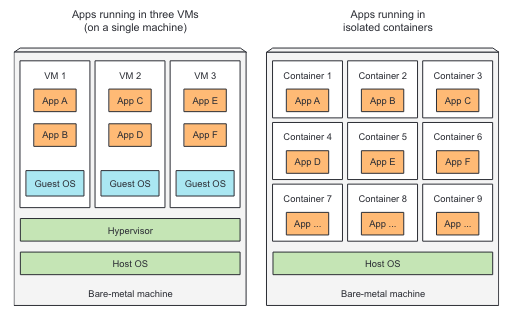
\includegraphics[width=\textwidth]{gfx/chapters/2_grundlagen/container-vs-vm.png}
  \caption{Virtualization vs. Container Technologie}
  \label{fig:container:vergleich}
  \source{\cite{Marko2018}}
\end{figure}

In \ref{fig:container:vergleich} wird der Unterschied von \acp{VM} und Containern dargestellt. 
Jede Anwendung wird innerhalb eines Containers betrieben, sodass eine vollständige Isolation der Prozesse
stattfinden kann \cite{Marko2018}.

Die Isolation von Containern findet mit der Nutzung von \emph{Linux Namespaces} und \emph{Linux Control Groups (cgroups)} statt \cite{Marko2018}.
Namespaces sorgen für die Isolation der Prozesse, 
während cgroups ein Limit für Ressourcen eines Prozesses festlegen können \cite{Marko2018}.

Container ermutigen Entwickler nach dem Konzept \emph{Immutable Infrastructure} zu arbeiten \cite{Burns2019}.
Das Immutable Infrastructure Prinzip besagt, dass sobald eine Version, beziehungsweise ein Artefakt, einer Softwarekomponente erstellt wird,
Nutzer keine Änderungen an diesem Artfakt vornehmen dürfen \cite{Burns2019}. 
Anstatt auf einem Server eine neue Version der Anwendung einzuspielen, werden neue Container Abbilder mit dem erstellen Artefakt gebaut, 
und der laufende Container mit dem neuen Abbild ersetzt \cite{Burns2019}.

\subsection{Docker}
Docker dient als Umgebung zum Verwalten, Erstellen und Betreiben von Containern \cite{Marko2018}.
Dabei besitzt Docker 3 grundliegende Konzepte:

\paragraph{Images}
Images sind Abbilder einer Anwendung und dessen Umgebung.
Es besitzt ein Dateisystem, sowie alle Dateien, die während des Erstellprozesses dem Image hinzugefügt wurden \cite{Marko2018}.

\paragraph{Registries}
Registries sind Speicherorte für Images. Sobald ein neues Image erstellt wird, kann es in eine Registry \emph{gepushed} werden,
um es für andere Systeme zur Verfügung zu stellen \cite{Marko2018}.

\paragraph{Container}
Docker Container sind reguläre Linux Container, die von einem Image erstellt wurden \cite{Marko2018}.